\section[检查观测值]{检查观测值\\Investigations of the Observations}
Before dealing with the complex code for Real-Time Kinematic (RTK) observations, we
split up into smaller steps I, II, and III. Various tools will demonstrate more ways of solving the larger problem: Estimate the baseline using code and phase .

\subsection{Ionospheric Delay}

\uppercase\expandafter{\romannumeral1}. From the basic equations (10.9) for $P_{1}$,$\Phi_{1}$,$P_{2}$,$\Phi_{2}$ we keep the second and fourth observations and remember that we are dealing with double differences:
\begin{equation}
\begin{split}
\Phi_{1}=\rho^{*}-I+\lambda_{1}N^{1}-\epsilon_{1}\\
\Phi_{2}=\rho^{*}-I+\lambda_{2}N^{2}-\epsilon_{2}
\end{split}
\end{equation}
Ignoring the error terms $\epsilon_{i}$ and eliminating $\rho^{*}$ gives an expression for the ionospheric delay
\begin{equation}
I=\frac{(\Phi_{2}-\lambda_{2}N_{2})-(\Phi_{1}-\lambda_{1}N_{1})}{1-\alpha}
\end{equation}

\begin{figure}
	\centering
	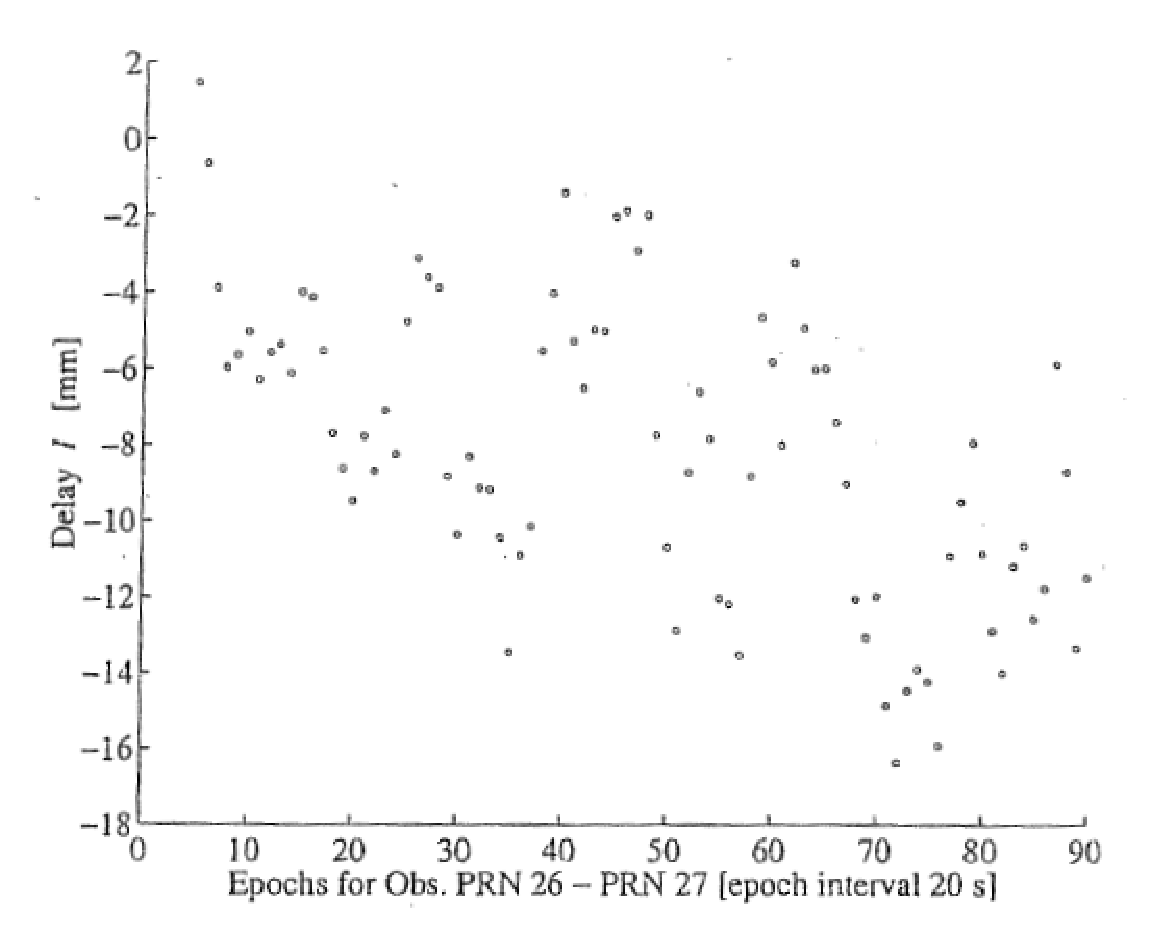
\includegraphics[width=0.4\linewidth]{TeX_files/Part03/chapter10/image/9-7}
	\caption{Ionospheric delay varying from 2 mm to -16mm for double differenced phases from (10.21). The baseline length is 4.6km.}
	\label{fig:9-7}
\end{figure}

This variable is plotted in Figure 10.7. It scatters within a few cm. So testing can determine if the condition I=0 (no delay) can be accepted or not.

We can eliminate the ionospheric term I from the two equations (10.20), to find
\begin{equation}
60\Phi_{1}/\lambda_{1}-77\Phi_{2}/\lambda_{2}=60N_{1}-77N_{2}
\end{equation}

The coefficients 60 and 77 appear because $\frac{f_{1}}{f_{2}}=\frac{154}{120}=\frac{77}{60}$.However, a drawback of the large coefficients 60 and 77 is that they amplify the noise.

\uppercase\expandafter{\romannumeral2}. Here is another way to eliminate I, using two frequencies. The ionospheric delay can vary from a few meters to tens of meters. Fortunately the ionosphere is dispersive:
the delay depends on the frequency f. From equation (10.8) we derive a dual frequency
ionospheric correction. Start with two pseudoranges on L1 and L2 at one satellite:
$$
P_{1}=\rho^{*}+I-e_{1}
$$
$$
P_{2}=\rho^{*}+\alpha I-e_{2}
$$\\
Ignoring the error terms $e_{i}$, and eliminating I, we get an ideal pseudorange $\rho^{*}$:
$$
\rho^{*}=P_{1}-\frac{P_{1}-P_{2}}{1-\alpha}=P_{1}+1.545727802(P_{1}-P_{2})
$$\\
This linear combination of pseudoranges can be called the ionosphere free combination.

\uppercase\expandafter{\romannumeral3}. Next we describe a simple filter $k_dd4$ that uses methods given in Chapter 8. It has four unknowns: the ideal pseudorange $\rho^{*}$, the delay I , and the integer ambiguities $N_{1}$ and $N_{2}$. We observe pseudorange P and code $\Phi$ on both frequencies, and repeat (10.9):
$$
\begin{bmatrix}
1&1&0&0\\
1&-1&\lambda_{1}&0\\
1&\alpha&0&0\\
1&-\alpha&0&\lambda_{2}
\end{bmatrix}
\begin{bmatrix}
\rho^{*}\\I\\N_{1}\\N_{2}
\end{bmatrix}
=
\begin{bmatrix}
P_{1}\\\Phi_{1}\\P_{2}\\\Phi_{2}
\end{bmatrix}
-e
$$\\
The variances for the independent $P_{1},\Phi_{1},P_{2},\Phi_{2}$ are $0.3^{2} , 0.005^{2} , 0.3^{2},$ and $0.005^{2} m^{2} $.The initial value for $x_{0}$ solves the four equations in the four unknowns at epoch 5. The early data are quite noisy, due to a cold start of the receiver. The variances for the errors $\epsilon$ in the state equation are 100, 10, 0, 0$m^{2}$ (for $\rho^{*}$ and I and the ambiguities). The output contains the filtered values for $\rho^{*}$,I,$N_{1}$ and the wide lane ambiguity $N_{w}=N_{1}-N^{2}$.

The ionospheric delay can change rapidly in absolute value. Variations depend on season , latitude, time of day, and other parameters. Extensive studies of the ionospheric delay have been reported in Klobuchar (1996).

\subsection{Tropospheric Delay}

Here is a model for the tropospheric delay T of GPS signals received at latitude $\varphi$ with a zenith distance z = $90^{\circ}$-h . The air pressure $P_{0}$ is in millibars, the height H is in km , the temperature $T_{0}$ is in $^{\circ}$K, and the partial pressure $e_{0}$ of water vapor is in millibars. Then
\begin{equation}
T=0.002277\frac{1+0.0026cos2\varphi+0.00028H}{cosz}(P_{0}+(\frac{1255}{T_{0}}+0.05)e_{0}).
\end{equation}\\
This simple model can been extended in various ways. As we only intend to determine
short baselines, and to an accuracy of cm-level, we have implemented the M-file tropo
which easily fulfills this demand . We compute the tropospheric zenith delay to be T$\approx$
2.4m . And we read from the formula that the delay grows inversely proportional to
cos z. In processing GPS observations you often select a cut-off angle of $15^{\circ}$.

The M-file tropo needs the following parameters as input:

- sinel  sine of elevation angle of satellite,

- hsta  height of station in km, p atmospheric pressure in mb at height hp,

- tkel  surface temperature in degrees Kelvin at height htkel,

- hum  humidity in \% at height hhum ,

- hp  height of pressure measurement in km ,

- htkel  height of temperature measurement in km,and

- hhum  height of humidity measurement in km.

The code tropo may compete even with the most precise and recent ones published.


The zenith delay is known to within about 2\% uncertainty or better. For zenith distances
smaller than  $75^{\circ}$ this uncertainty does not increase very much. If all pseudoranges have a constant bias this would not affect the position calculation but just add to the receiver clock offset. If the tropospheric delay T is not constant this can affect the height of the point. Yet , in double differencing for short baselines this is not a serious error.

\subsection{Multipath on Code Observations}

Multipath describes the situation where signals coming from the satellite propagate along
several paths to the receiver antenna. The main part of the signal arrives directly from the satellite, but part of the signal is reflected from a nearby surface. Multipath depends on satellite geometry and the antenna environment, and is difficult to model. For long observation periods��24 hours��the multipath effects are partly reduced by averaging. For short observation periods, multipath is a serious problem.

For more details on how to compute the multipath delay, see page\textbf{ 291,need to find the right page}.

\subsection{Bayes Filter for Ambiguity Estimation}

We now return to a single one-way range between a satellite and a receiver. We assume that P-code pseudoranges and phase observations are taken on both frequencies L1 and L2 for 50 epochs. As usual we denote the observations by $P_{1}$,$\Phi_{1}$,$P_{2}$,and $\Phi_{2}$. Unlike all earlier instances, the observations are undifferenced! Our goal is to study how well P code pseudoranges can help to estimate ambiguities $N_{1} - N_{2}$ and $N_{1}$ for undifferenced observations. We describe ideas published in Euler \& Goad(1991).

An appropriate Kalman filter is a sequential formulation of the Bayes version:

\begin{equation}
State \, \, prediction \, \, \hat{x}_{k|k-1}=F_{k-1}\hat{x}_{k-1|k-1}
\end{equation}
\begin{equation}
Covariance \, \, prediction \, \, P_{k|k-1}=F_{k-1}P_{k-1|k-1}F_{k-1}^{T}+\Sigma_{\epsilon,k}
\end{equation}
\begin{equation}
Covariance \, \, update \, \,P_{k|k}=(P_{k|k-1}^{-1}+A_{k}^{T}\Sigma_{e,k}^{-1}A_{k})^{-1}
\end{equation}
\begin{equation}
Gain \, \, matrix (after\,P_{k|k}!)\, \,  \hat{x}_{k|k-1}=F_{k-1}\hat{x}_{k-1|k-1}
\end{equation}
\begin{equation}
State \, \, update \, \,\hat{x}_{k|k}=\hat{x}_{k|k-1}+K_{k}(b_{k}-A_{k}\hat{x}_{k|k-1}).
\end{equation}

A remark is needed on the matrix $P_{k|k-1}^{-1}$ in (10.27). In case the state transition noise is large in (10.25), it is difficult to predict the corresponding entry of the state vector $\hat{x}_{k|k}$.This situation is handled well by the predicted covariance
$P_{k|k-1}=\begin{bmatrix}
\infty & \sigma_{12} \\
\sigma_{21} & \sigma_{22}\end{bmatrix}$.
Here denotes one very large variance, or a submatrix with almost infinite diagonal elements.

The inverse of this (block) matrix has the following form by the matrix identity (8.45):
$$
Singular case \,\,P_{k|k-1}^{-1}=\begin{bmatrix}
0 & 0\\
0 & \sigma_{22}^{-1}\end{bmatrix}
$$

This implies that the first entries of the previous state vector x will have no influence on the new state. The filter process that we now describe takes advantage of this behavior.

Our observation equations $b_{k}=A_{k}x_{k}-e_{k}$ are still identical to (10.9):
$$
\begin{bmatrix}
P_{1}\\\Phi_{1}\\P_{2}\\\Phi_{2}
\end{bmatrix}
=\begin{bmatrix}
1&1&0&0\\
1&-1&\lambda_{1}&0\\
1&\alpha&0&0\\
1&-\alpha&0&\lambda_{2}
\end{bmatrix}
\begin{bmatrix}
\rho^{*}\\I\\N_{1}\\N_{2}
\end{bmatrix}
-noise
$$

\begin{table}[htbp]
	\caption{Standard deviation $\sigma_{P}$ for one-way ranges as function of elevation angle h}
	\begin{tabular}{lllllllllll}
		\hline
		$h[^{\circ}]$ & 0 & 10 & 20 & 30 & 40 & 50 & 60 & 70 & 80 & 90\\
		\hline
		$\sigma_{P}[m]$ & 4.58 & 1.73 & 0.69 & 0.30 & 0.16 & 0.11 & 0.09 & 0.08 & 0.08 & 0.08\\
		\hline
	\end{tabular}
\end{table}

The system equation is the steady model $\hat{x}_{k|k-1}=\hat{x}_{k-1|k-1}$ (constant state equation). Weuse the Kalman filter with $F_{k}=I$, and (10.26) becomes $P_{k|k-1}=P_{k-1|k-1}+\Sigma_{\epsilon,k}$.The transition covariance matrix $\Sigma_{\epsilon,k}$ is diagonal. The (3,3) and (4,4) entries must be zero to prevent $N_{1}$ and $N_{2}$ from changing. We have to allow for large changes of $\rho^{*}$ and I:
$$
\Sigma_{\epsilon,k}=
\begin{bmatrix}
\infty \\
&\infty \\
&&0\\
&&&0
\end{bmatrix}
$$\\
Again $\infty$ symbolizes a very large but finite number. The prediction from (10.26) is






\begin{equation}
P_{k|k-1}=P_{k-1|k-1}+\Sigma_{\epsilon,k}=
\begin{bmatrix}
\infty & \sigma_{12} & \sigma_{13} & \sigma_{14}\\
\sigma_{21} & \infty & \sigma_{23} & \sigma_{24}\\
\hline
\sigma_{31} & \sigma_{32}& \sigma_{33} & \sigma_{34}\\
\sigma_{41} & \sigma_{42}& \sigma_{43} & \sigma_{44}
\end{bmatrix}
\end{equation}
According to (8.42) and (8.43) we get this further singular case:
$$
P_{k|k-1}^{-1}=
\begin{bmatrix}
\begin{matrix}
0&0\\
0&0
\end{matrix}
\begin{matrix}
0&0\\
0&0
\end{matrix}\\
\begin{matrix}
0&0\\
0&0
\end{matrix}
\begin{bmatrix}
\sigma_{33} & \sigma_{34}\\
\sigma_{43} & \sigma_{44}
\end{bmatrix}^{-1}
\end{bmatrix}
$$




This means that previous information of $\rho^{*}$ and I is effectively neglected in the update of the new state vector $\hat{x}_{k|k}$. The covariance matrix of the observations $b_{k}$ is
\begin{equation}
\Sigma_{e,k}=
\begin{bmatrix}
\sigma_{P_{1}}^{2}\\
&\sigma_{\Phi_{1}}^{2}\\
&&\sigma_{P{2}}^{2}\\
&&&\sigma_{\Phi_{2}}^{2}
\end{bmatrix}
=
\begin{bmatrix}
\sigma_{P_{1}}^{2}\\
&0.005^{2}\\
&&\sigma_{P{2}}^{2}\\
&&&0.005^{2}
\end{bmatrix}
\end{equation}
Uncertainties depending on elevation can be modeled as an exponential expression for the standard error $\sigma_{P}=a_{0}+a_{1}e^{-h/h_{0}}$ , where $h_{0}$ is a scaled value of the elevation error. The constants $a_{0}$ and $a_{1}$ are receiver dependent and must be estimated empirically. Section 5.3 provides methods for estimating $a_{0}$ and $a_{1}$. Reasonable values are $a_{0}$ = 0.08m, $a_{1}$ = 4.5m and $h_{0}$ = $10^{\circ}$. This gives the elevation uncertainty in meters:
$$
Elevation uncertainty \,\, \sigma_{P}=0.08+4.5e^{-h/10}
$$
with h in degrees, tabulated in Table 10.1. To repeat, $\sigma_{P}^{2}$ yields the entries (1,1) and (3,3) of $\Sigma_{e,k}$.Phase measurements are considered to be independent of elevation angle.
\begin{table}[htbp]
	\caption{Eigenvalues of covariance matrix for narrow and wide lane ambiguities}
	\begin{tabular}{llll}
		\hline
		PRN & mean of h & $\lambda_{max}$ & $\lambda_{min}$ \\
		\hline
		2 & 60 & 0,276 & 0.00007\\
		9 & 18 & 15.594 & 0.00348\\
		16 & 20& 7.424 &0.00166 \\
		23&20&12.010&0.00268 \\
		26&70&0.235&0.00006\\
		27&30&3.241&0.00073\\
		\hline
	\end{tabular}
\end{table}

The estimated values for the wide lane ambiguity $N_{w}=N_{1}-N_{2}$ were used to form double difference ambiguities $N_{w,ij}^{kl}=(N_{w,i}^{k}-N_{w,i}^{l})-(N_{w,j}^{k}-N_{w,j}^{l})$ In a11 cases the computed values were in agreement with the��exact��values. So a good way of estimating double difference ambiguities is to start from the one-way ambiguities. The estimates of one-way ambiguities are independent of the length of the baseline. These cases can avoid a computational need for a LAMBDA method.

A similar procedure for $N_{1}$ ambiguity shows that in this case the computed double difference ambiguities never deviate more than two cycles from the true values . This is a really promising procedure: simpler than others.

From the filter covariance matrix $P_{N|N}$ we can compute the covariance matrix for the��wide��and��narrow��combinations $N_{w}=N_{1}-N_{2}$ and $N_{n}=N_{1}+N_{2}$. The smallest eigenvalue $N_{1}-N_{2}$ in Table 10.2 shows the standard deviation of $\lambda_{min}$. The smaller it is, the more reliable is the computation. Recall that the wide lane has wave length $\lambda_{w}$ = 0.863 m (from  $1/\lambda_{w}=1/\lambda_{1}-1/\lambda_{2}$) and the narrow lane has $\lambda_{n}$ = 0.107 m (from $1/\lambda_{n}=1/\lambda_{1}+1/\lambda_{2}$). To estimate the standard deviation $\sigma_{w}$ of the wide lane ambiguity we use $\sigma_{w}=\sqrt{\lambda_{min}}\lambda_{w}$ = 0.05 m. The largest eigenvalue $\lambda_{max}$ measures the difficulty in estimating $N_{1}+N_{2}$. A similar calculation yields $\sigma_{n}=\sqrt{\lambda_{max}}\lambda_{n}$ = 0.49 m which is more than four times $\lambda_{n}$! This explains why it is always more difficult to calculate the narrow lane ambiguity $N_{1}+N_{2}$.

\begin{table}[htbp]
	\caption{Ambiguities estimated by filtering one-ways. SD and DD are single and
		double difference.}
	\newcommand{\tabincell}[2]{\begin{tabular}{@{}#1@{}}#2\end{tabular}}
	\begin{tabular}{cccccccc}
		\hline
		PRN & \tabincell{c}{Linear \\Comb} & Master M  & Rover R & SD=M-R &\tabincell{c}{DD=\\$ SD_{26}-SD_{i}$}&Exact DD & \tabincell{c}{Elevation\\$[^{\circ}]$} \\
		\hline
		2 & $N_{1}-N_{2}$ & -27965804.3 & -24897335.6 &-3068468.7&-104539.9&-104540&59-61\\
		&$N_{1}$ &-126566312.1 &-112753467.5 &-13812844.6& -458650.7 &-458650&\\
		9 & $N_{1}-N_{2}$ & -30299948.8 &-28466967.2 &-1832981.6 &-1340027.0 &-1340027 &14-25\\
		&$N_{1}$ & -137064692.1 & -128875084.1 &-8189608.0 &-6081887.3 &-6081889&\\
		16 & $N_{1}-N_{2}$ &-25853811.1&-26599158.2&745347.1&-3918355.7&-3918356 &30-17\\
		&$N_{1}$ &-117099419.5&-120568534.1& 3469114.6&-17740609.9 &-17740609&\\
		23& $N_{1}-N_{2}$ &-31520321.4&-28336205.6&-3184115.8&11107.2&11107 &17-25 \\
		&$N_{1}$ &-141013589.3&-128295732.5 &-12717856.8&-1553638.5&-1553637&\\
		26& $N_{1}-N_{2}$&-27574563.2 &-24401554.6&-3173008.6& & &66-75\\
		&$N_{1}$ &-124770191.1 &-110498695.8& -14271495.3& & &\\
		27& $N_{1}-N_{2}$&-25222330.2&-25755098.4&532768.2 &-3705776.8 &-3705777&35-23\\
		&$N_{1}$&-114238281.7&-116723571.7&2485290.0&-16756785.3&-16756785&\\
		\hline
	\end{tabular}
\end{table}

By running the M-file one\_way we get the estimates presented in Table 10.3. Single differences are defined as master values minus rover values. For the double differences we select PRN 26 as the reference satellite. This PRN has largest average elevation angle. All rounded values of wide-lane ambiguities are correct while some $N_{1}$ ambiguities deviate up to two cycles for PRN��s with low elevation angles, viz.9 and 23.

The exact double differences in the second last column are output from the M-file
ash\_base. Independently those values are checked by a commercial software.